\chapter{Create your first Drupal site}

\section{Acquia Dev Desktop}

As mentioned before we will be managing our local Drupal installation through the Acquia Dev Desktop tool. The tool contains a PHP hosting environment which includes: the PHP runtime, an Apache web server, a MySQL database server and phpMyAdmin for database management. 

Figure \ref{fig:acquia_dev_desktop_interface} shows the Acquia Dev Desktop interface. On the left you can see an overview of the sites you created. The plus and minus signs in the bottom left corner allow you to add or remove a Drupal site.
In the right panel you can see the information of the site you selected. It contains the following:
\begin{description}
	\item[Local site] The local url to your site. Refers to the local Apache server running on port 8083.
	\item[Local code] Shows the path to the local codebase. All the code your site uses is stored in this location on your computer.
	\item[Local database] A link to the phpMyAdmin page of your local database.
	\item[PHP version] The PHP version your site uses, we will use the default version (5.5.27).
\end{description}


	\begin{figure}[H]
		\centering
		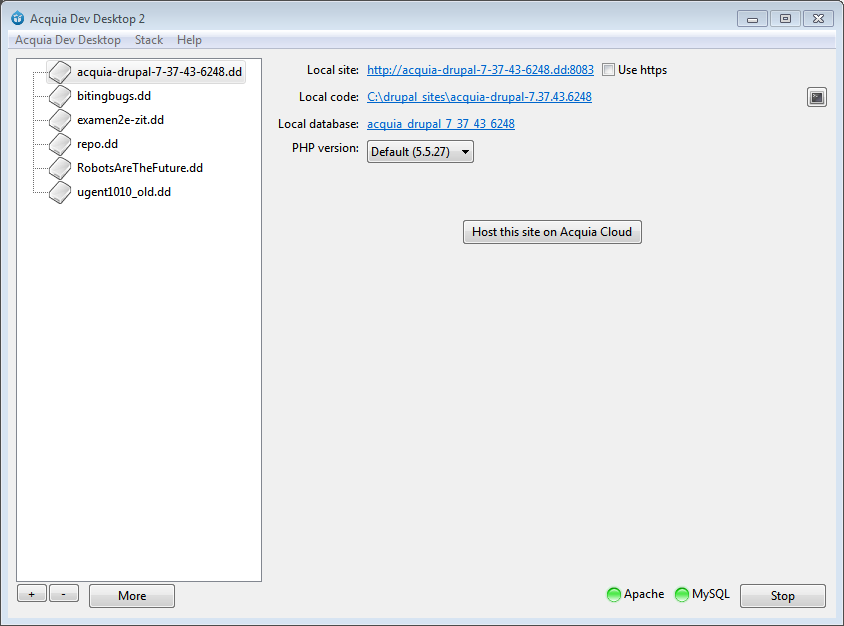
\includegraphics[width=\textwidth]{chapter3/acquia_dev_desktop_interface}
		\caption{The Acquia Dev Desktop interface}
		\label{fig:acquia_dev_desktop_interface}
	\end{figure}
	
\section{Creating a new site}

To create a new site through Acquia Dev Desktop, click the plus button in the bottom left corner. Select \textbf{New Drupal site...} in the context menu (Figure \ref{fig:acquia_dev_desktop_new_site_context_menu})

\begin{figure}[H]
	\centering
	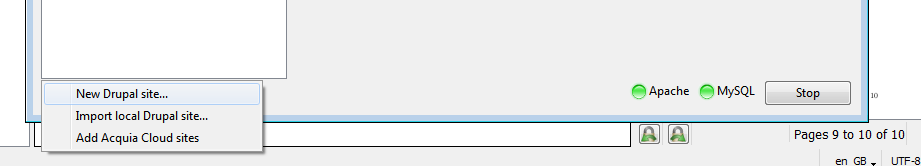
\includegraphics[width=\textwidth]{chapter3/acquia_dev_desktop_new_site_context_menu}
	\caption{New site menu}
	\label{fig:acquia_dev_desktop_new_site_context_menu}
\end{figure}

In the next window you will see an overview of different standard Drupal installations. Select the Drupal 8 version (Figure \ref{fig:acquia_dev_desktop_druppal_installations})

 \begin{figure}[H]
 	\centering
 	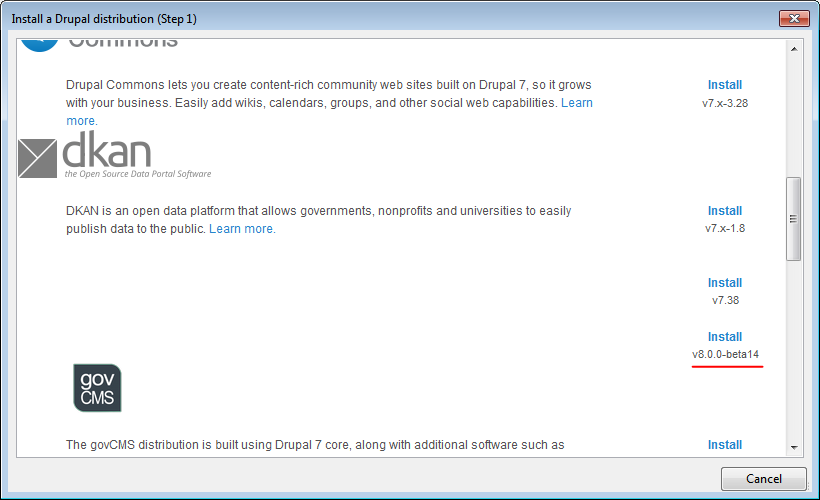
\includegraphics[width=\textwidth]{chapter3/acquia_dev_desktop_druppal_installations}
 	\caption{Drupal version selection}
 	\label{fig:acquia_dev_desktop_druppal_installations}
 \end{figure}
 
 Fill out the following site information in the next window (Figure \ref{fig:acquia_dev_desktop_new_site_configuration}). Note that if you have configured Acquia Dev Desktop to store your sites in a different location the default path might not be \url{C:\drupal_sites\}.
 
  \begin{figure}[H]
  	\centering
  	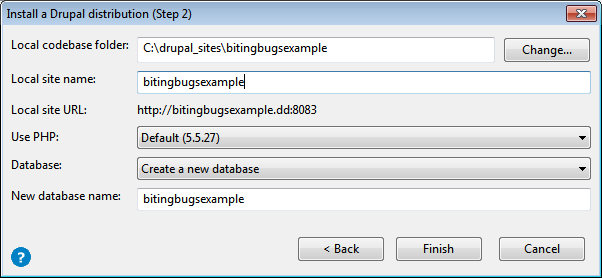
\includegraphics[width=\textwidth]{chapter3/acquia_dev_desktop_new_site_configuration}
  	\caption{Site configuration}
  	\label{fig:acquia_dev_desktop_new_site_configuration}
  \end{figure}
  
  Click \textbf{Finish}. Acquia Dev Desktop unpacks the selected Drupal 8 archive into the local codebase folder. When the process finishes click the link to your local site in the right panel of the Acquia Dev Desktop, this will open the installation page for your site in your default browser (Figure \ref{fig:drupal_site_install_p1}).
  
  \begin{figure}[H]
  	\centering
  	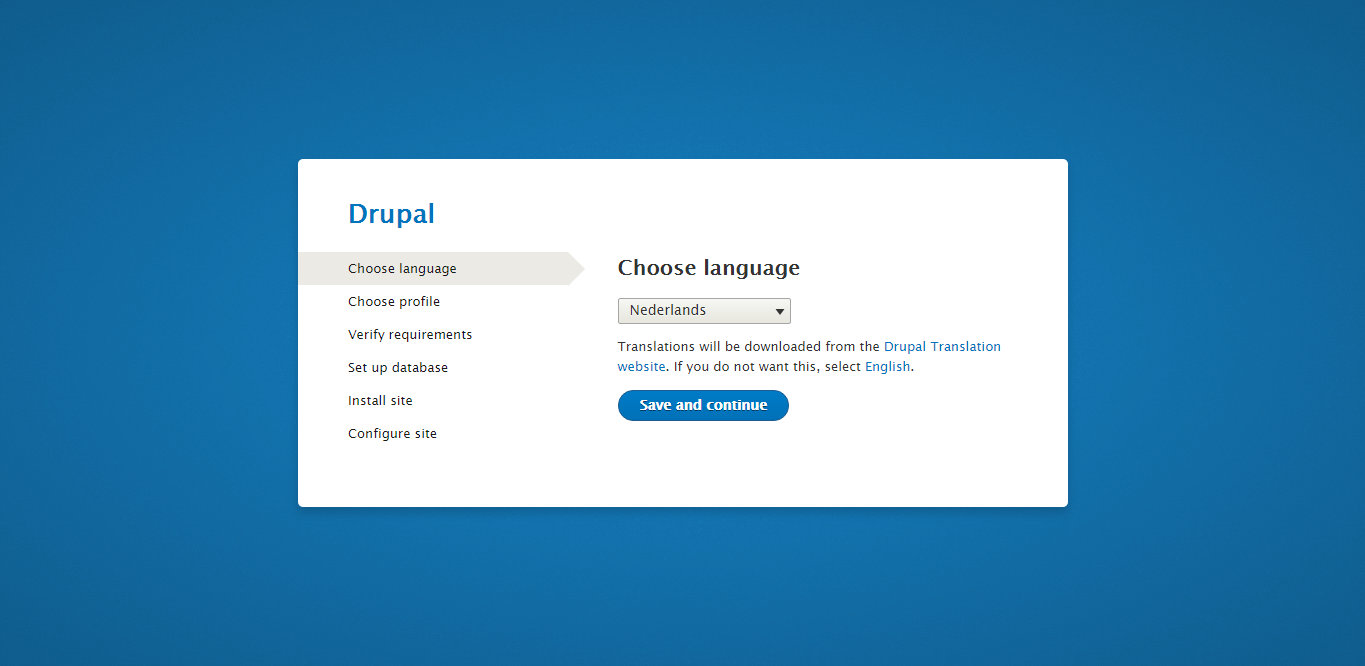
\includegraphics[width=\textwidth]{chapter3/drupal_site_install_p1}
  	\caption{Site installation: Choose language}
  	\label{fig:drupal_site_install_p1}
  \end{figure}
  
  Since this course is in English we'll select it as our default site language. Click \textbf{Save} and on the next page select the \textbf{Standard} installation profile (Figure \ref{fig:drupal_site_install_p2}).
  
  \begin{figure}[H]
  	\centering
  	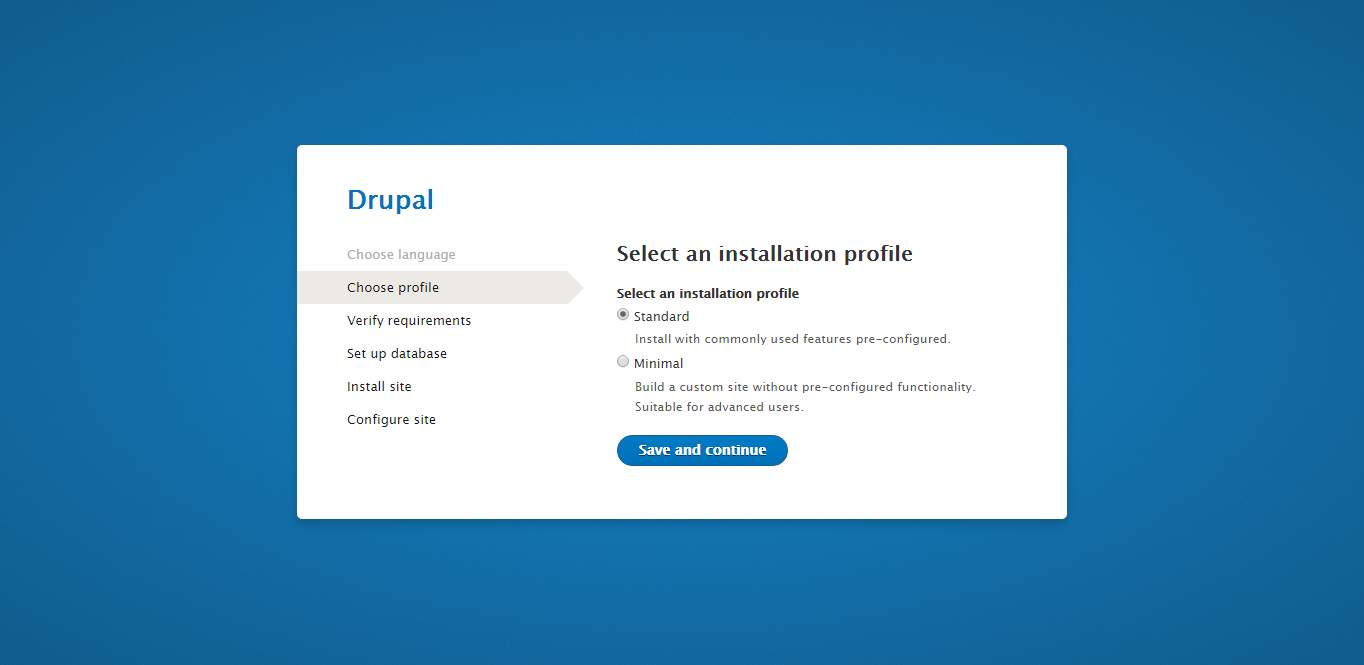
\includegraphics[width=\textwidth]{chapter3/drupal_site_install_p2}
  	\caption{Site installation: installation profile}
  	\label{fig:drupal_site_install_p2}
  \end{figure}
  
  Click \textbf{Save and continue} This step might take a few minutes. After the installation has finished we need to configure some site properties. Enter the following information (Figure \ref{fig:drupal_site_install_p3} and \ref{fig:drupal_site_install_p4}):
  
  \begin{description}
  	\item[Site name:] bitingbugsexample
  	\item[Site email address:] noreply@bitingbugsexample.com
  	\item[Username:] drupal
  	\item[Password:] Drupal
  	\item[Confirm password:] Drupal
  	\item[Email address:] info@bitingbugsexample.com
  	\item[Default country:] Belgium
  	\item[Default time zone:] Europe/Brussels
  \end{description}
  
  After entering the right configuration you can click the \textbf{Save and continue} button.
  
  \begin{figure}[H]
  	\centering
  	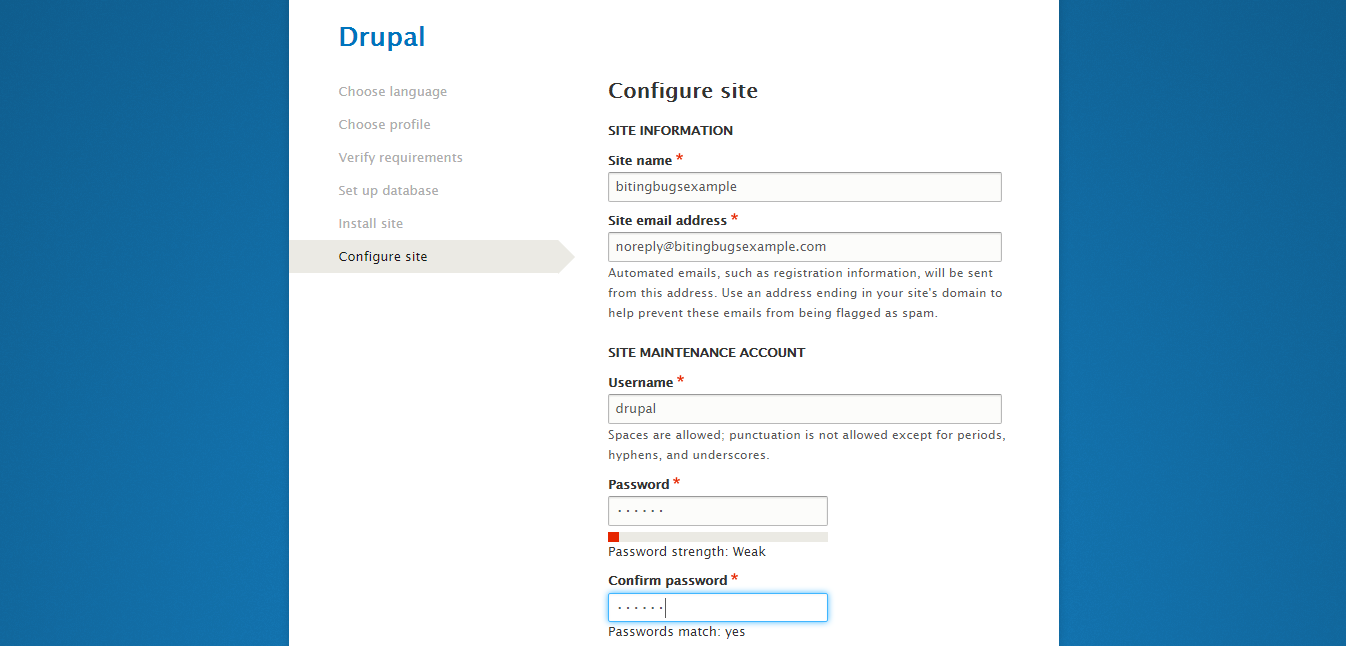
\includegraphics[width=\textwidth]{chapter3/drupal_site_install_p3}
  	\caption{Site installation: installation configuration 1}
  	\label{fig:drupal_site_install_p3}
  \end{figure}
  \begin{figure}[H]
  	\centering
  	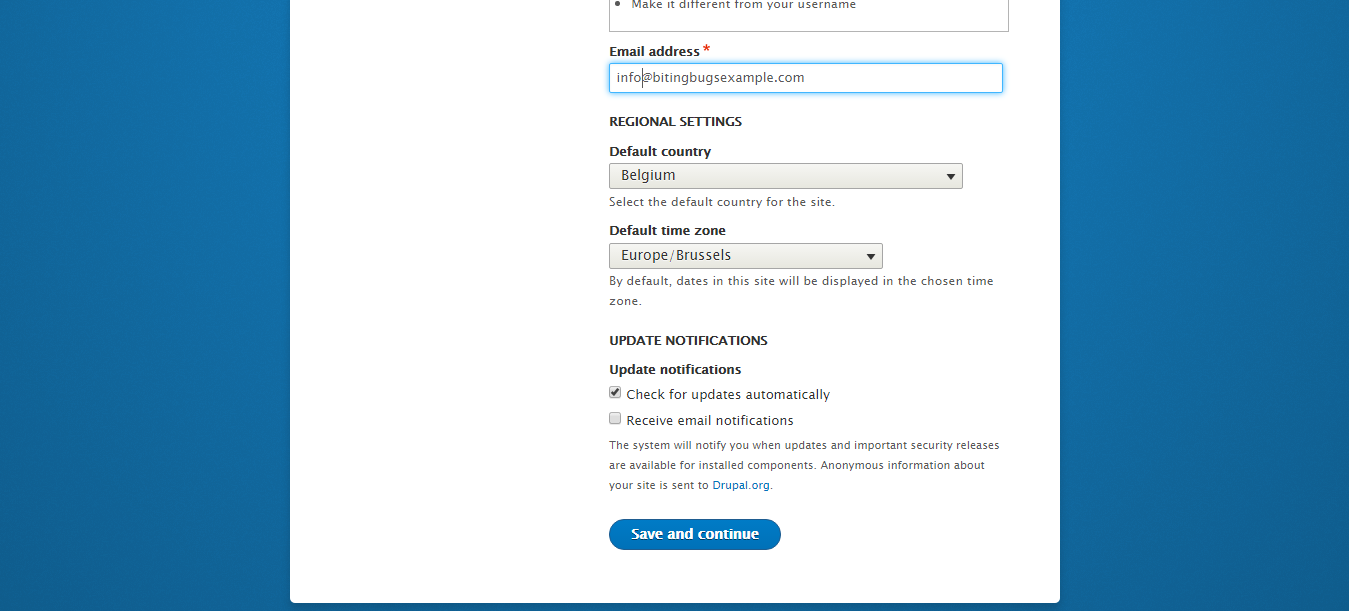
\includegraphics[width=\textwidth]{chapter3/drupal_site_install_p4}
  	\caption{Site installation: installation configuration 2}
  	\label{fig:drupal_site_install_p4}
  \end{figure}
  
  Et voila, you have your first Drupal site. It's pretty basic, you only have a welcome page, no content yet. By default, after completing the installation, you are logged in as administrator (figure \ref{fig:first_drupal_site}). To see the non administrator layout click the \textbf{Log out} link in the top right corner. As you can see we only have a basic one page site with our site title at the top. Now log back into your site with username: drupal and password: Drupal.
  
  
  \begin{figure}[H]
  	\centering
  	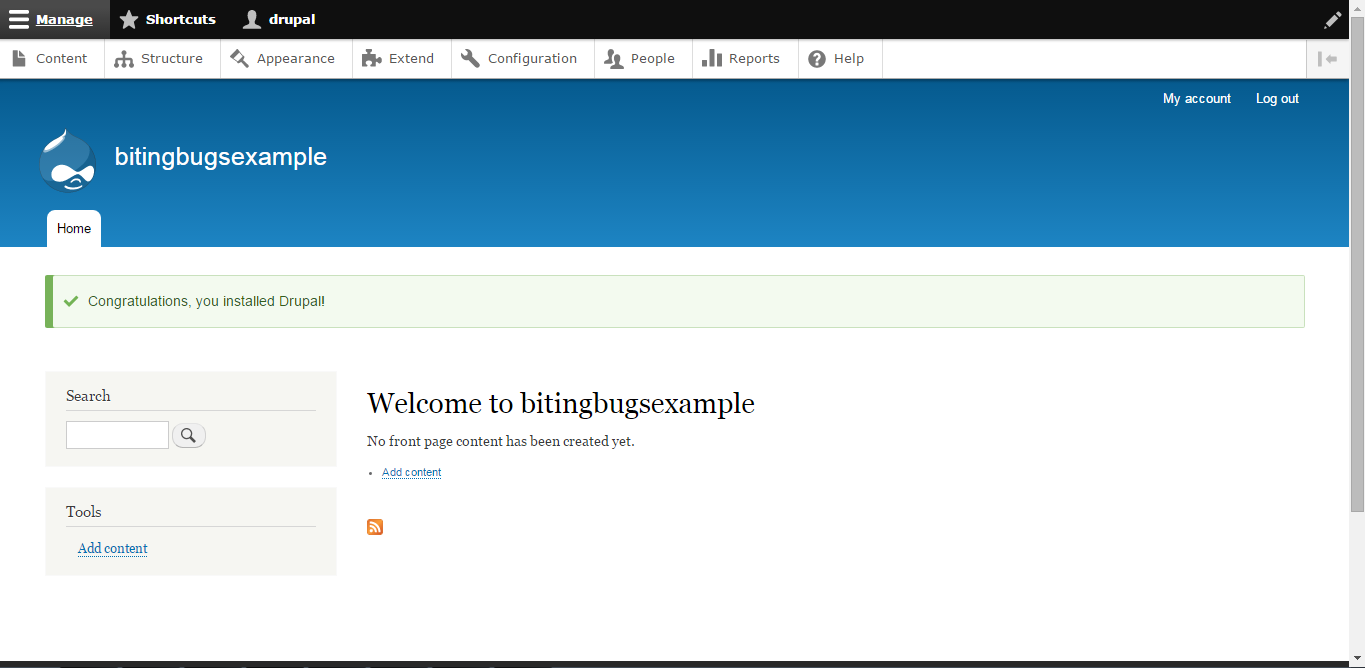
\includegraphics[width=\textwidth]{chapter3/first_drupal_site}
  	\caption{Your first Drupal site.}
  	\label{fig:first_drupal_site}
  \end{figure}
  
  \section{review exercises}
  
  Create a new Drupal 8 site with the following properties:
  
   \begin{description}
   	\item[Sitename] exploringdrupal8
   	\item[database] exploringdrupal8
   	\item[Language] English
   	\item[Username] drupal, password: Drupal
   	\item[Timezone] Europe/Brussels
   	\item[Country] Belgium
   \end{description}
  
	
